
\section{Théorie des Graphes}

\subsection{Définitions}

\begin{defn}
Un graphe $\Gamma$ est un triplet $(V,E,\gamma)$ où V est un ensemble fini dont les éléments sont appelés sommets, E est un ensemble fini dont les éléments sont appelés arêtes, $\gamma$ est une fonction $\gamma : E \rightarrow Paires(V)$. On nottera le plus souvent $\Gamma = (V,E)$ en omettant la fonction $\gamma$.\\

Soit $\gamma(e) = \{x,y\}$ pour $e \in E, x,y \in V$:
\begin{center}
	\begin{enumerate}
	\item On dit que x et y sont adjacents.

	\item On dit que e est incidente à x et y. \\
	\end{enumerate}
\end{center}

\end{defn}

\begin{defn}
Soit $\Gamma = (V,E,\gamma)$ un graphe.

\begin{enumerate}
\item $\gamma(e)= \{x,x\}$ pour $e \in E, x \in V$ est appellé un lacet.
\item Si au moins 2 arêtes sont incidentes à 2 mêmes somments, on les appelle arêtes multiples.
\item Un graphe est simple s'il n'a ni lacet, ni arêtes multiples. Dans ce cas, on omet la fonction $\gamma$,on note $\Gamma = (V,E)$ et E est identifié un sous-ensemble de Paires(V). \\
\end{enumerate}
\end{defn}

\begin{defn}
Soit $\Gamma = (V,E)$ un graphe. Le degré d'un sommet $v \in V$ est le nombre d'arêtes incidentes à v, les lacets comptant pour 2 arêtes. On note le degré de v par deg(V).
\end{defn}

\begin{exmp}
Dans la figure suivante, nous avons 2 sommets de degré 4 et 6 sommets de degré 1.
\end{exmp}

\begin{figure}[htb]
	\centering
	\begin{tikzpicture}[>=stealth',shorten >=1pt,auto,node distance=1.5cm,thick,main node/.style={circle,fill=blue!20,draw,font=\sffamily\large\bfseries}]

	\node[main node] (c1) {C};
	\node[main node] (c2) [right of=c1] {C};
	\node[main node] (h1) [above of=c1] {H};
	\node[main node] (h2) [left of=c1] {H};
	\node[main node] (h3) [below of=c1] {H};
	\node[main node] (h4) [above of=c2] {H};
	\node[main node] (h5) [right of=c2] {H};
	\node[main node] (h6) [below of=c2] {H};

	\path[every node/.style={font=\sffamily\small}]
	(c1) edge node [above] {} (h1)
		 edge node [left] {} (h2)
		 edge node [below] {} (h3)
		 edge node [right] {} (c2)
	(c2) edge node [above] {} (h4)
		 edge node [right] {} (h5)
		 edge node [below] {} (h6) ;

	\end{tikzpicture}

	\caption{Exemple degrés des sommets dans la molécule $C_{2}H_{6}$.}
\end{figure}

\begin{thrm}
Soit $\Gamma = (V,E)$, alors $$\sum_{i=1}^{\#V} deg(v_{i}) = 2\#E$$
\end{thrm}

\begin{demo}
Chaque arête contribue 2 fois dans la somme des degrés.
\end{demo}

\begin{corll}
La somme des degrés des sommets d'un graphe est paire. \\
\end{corll}

\begin{defn}
Le graphe complet $K_{n}$ est le graphe simple à n sommets pour lequel chaque paire de sommets est une arête.
\end{defn}

\begin{exmp}
	\begin{minipage}{.2\textwidth}
		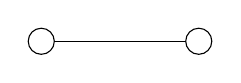
\begin{tikzpicture}
		 \def \radius {1cm}
		 \def \margin {8}
		 \def \n {2}
		 \foreach \s in {1,...,\n}
		  \node[draw, circle] (\s) at ({360/\n * (\s - 1)}:\radius) {};
		 \foreach \s in {1,...,\n}
		  \foreach \t in {\s,...,\n}
		   \draw (\t) -- (\s);
		\end{tikzpicture}
	\end{minipage}
	\begin{minipage}{.2\textwidth}
		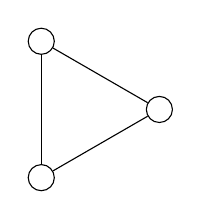
\begin{tikzpicture}
		 \def \radius {1cm}
		 \def \margin {8}
		 \def \n {3}
		 \foreach \s in {1,...,\n}
		  \node[draw, circle] (\s) at ({360/\n * (\s - 1)}:\radius) {};
		 \foreach \s in {1,...,\n}
		  \foreach \t in {\s,...,\n}
		   \draw (\t) -- (\s);
		\end{tikzpicture}
	\end{minipage}
	\begin{minipage}{.2\textwidth}
		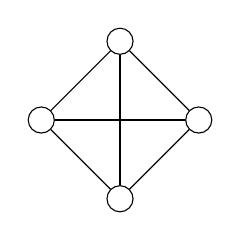
\begin{tikzpicture}
		 \def \radius {1cm}
		 \def \margin {8}
		 \def \n {4}
		 \foreach \s in {1,...,\n}
		  \node[draw, circle] (\s) at ({360/\n * (\s - 1)}:\radius) {};
		 \foreach \s in {1,...,\n}
		  \foreach \t in {\s,...,\n}
		   \draw (\t) -- (\s);
		\end{tikzpicture}
	\end{minipage}
	\begin{minipage}{.2\textwidth}
		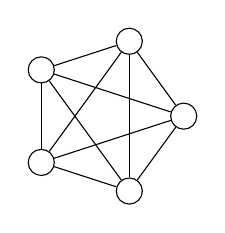
\begin{tikzpicture}
		 \def \radius {1cm}
		 \def \margin {8}
		 \def \n {5}
		 \foreach \s in {1,...,\n}
		  \node[draw, circle] (\s) at ({360/\n * (\s - 1)}:\radius) {};
		 \foreach \s in {1,...,\n}
		  \foreach \t in {\s,...,\n}
		   \draw (\t) -- (\s);
		\end{tikzpicture}
	\end{minipage}
	\begin{minipage}{.2\textwidth}
		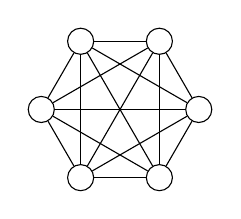
\begin{tikzpicture}
		 \def \radius {1cm}
		 \def \margin {8}
		 \def \n {6}
		 \foreach \s in {1,...,\n}
		  \node[draw, circle] (\s) at ({360/\n * (\s - 1)}:\radius) {};
		 \foreach \s in {1,...,\n}
		  \foreach \t in {\s,...,\n}
		   \draw (\t) -- (\s);
		\end{tikzpicture}
	\end{minipage}
\end{exmp}

\begin{defn}
Un graphe ${\Gamma}'=(U,F)$ est un sous-graphe de $\Gamma=(V,E)$ si $ U \subseteq V$ et $F \subseteq E$. On nottera $ {\Gamma}' \leq \Gamma$.
\end{defn}

\begin{exmp}
$ K_{m} \leq K_{n}$ si $ m \leq n$.
\end{exmp}

\begin{exo}
Montrer que $K_{m}$ possède $ q=\frac{1}{2}n(n-1)$ arêtes.
\end{exo}

%----------------------------------------------------

\subsection{Chemins dans les graphes}

\begin{defn}
Soit $\Gamma = (V,E)$ et $v,w \in V$. Un chemin de v à w de longueur n est une séquence alternée de $(n+1)$ sommets $v_{0},v_{1},...,v_{n}$ et de n arêtes $e_{1},e_{2},...,e_{n}$ de la forme $$ (v_{0},e_{1},v_{1},e_{2},...,e_{n},v_{n})$$ dans laquelle chaque $e_{i}$ est incident à $v_{i-1}$ et $v_{i}$ pour $1 \leq i \leq n$ et $ e_{i} \neq e_{j} , \forall i \neq j \in 1,...,n$ \\

Un chemin est simple si aucun sommet ne se répète sauf peut-être $v_{0}$ et $v_{n}$. \\

Dans un graphe simple on nottera juste la suite des sommets lorsque l'on décrit un chemin. \\

\end{defn}

\begin{defn}
Un graphe $\Gamma = (V,E)$ est connexe si $\forall x,y \in V : \exists $ un chemin de x à y. \\

La composante connexe de $\Gamma$ contenant x est le sous-graphe ${\Gamma}'$ de $\Gamma$ dont les sommets et les arêtes sont contenus dans un chemin de $\Gamma$ démarrant en x. \\
\end{defn}

\begin{defn}
Soit $\Gamma = (V,E)$ et $v \in V$.\\

Un cycle est un chemin de v à v.\\

Un cycle simple est un cycle de v à v dans lequel aucun sommet n'est répété (mis à part le départ et l'arrivée).\\
\end{defn}

%----------------------------------------------------

\subsection{Arbres}

\begin{defn}
Un arbre est un graphe simple connexe qui ne contient aucun cycle.\\
\end{defn}

\begin{defn}
Dans un arbre, les sommets de degré 1 sont appellés les feuilles.\\
\end{defn}

\begin{exmp}
<Dessin Arbre>
\end{exmp}

\begin{prop}
Si T est un arbre avec $p\geq2$ sommets, alors T contient au moins 2 feuilles.
\end{prop}

\begin{demo}
T a p sommets. Tous les chemins sont de longueur inférieure ou égale à p. Considérons un chemin $v_{0},v_{1},...,v_{r}$ pour $v_{i} \in V$, $i=0,...,r$ de longueur maximale. Alors, $v_{0}$ et $v_{r}$ sont de degré 1.\\
\end{demo}

\begin{thrm}
Soit T un graphe simple à p sommets. Alors les 3 assertions suivantes sont équivalentes:
	\begin{enumerate}
	\item T est un arbre.
	\item T a $(p-1)$ arêtes et aucun cycle.
	\item T a $(p-1)$ arêtes et est connexe.
	\end{enumerate}
\end{thrm}

\begin{demo}
<Démonstration en 2 parties>.
\end{demo}

%----------------------------------------------------

\newpage
<-- COURS 2 MISSING -->
\newpage

\begin{thrm}[Dirac 1950]
Soit $\Gamma = (V,E)$ un graphe simple avec $p \geq 3$ sommets. Si $\forall v \in V: deg(v) \geq \frac{1}{2}p$, alors $\Gamma$ est Hamiltonien.
\end{thrm}

\begin{demo}
$\Gamma$ est connexe. Soit C = $(v_{0},v_{1},...,v_{k})$ un plus long chemin simple dans $\Gamma$ avec $v_{0} \neq v_{k}, k < p$.\\

$ deg(v_{0}) \geq \frac{p}{2}$, tous les sommets adjacents à $v_{0}$ sont dans $\{v_{1},...,v_{k}\}$\\

$ deg(v_{k}) \geq \frac{p}{2}$, tous les sommets adjacents à $v_{k}$ sont dans $\{v_{0},...,v_{k-1}\}$\\

Comme $k < q$, il doit exister $i \in \{0,...,k-1\}$ tel que $\{v_{i},v_{k}\} \in E$ et $\{v_{0},v_{i+1}\} \in E$. On obtient un cycle $\widetilde{C} = (v_{0},v_{1},...,v_{i},v_{k},v_{k-1},...,v_{i+1},v_{0})$ \\

\begin{figure}[htb]
	\centering
	\begin{tikzpicture}[mydot/.style={fill,circle,inner sep=2pt},]

		\node[mydot,label={$v_{0}$}] (v0) {};
		\node[mydot,below right=of v0] (v1) {};
		\node[mydot,above right=of v1] (v2) {};
		\node[mydot,below right=of v2,label={$v_{i}$}] (v3) {};
		\node[mydot,above right=of v3,label={$v_{i+1}$}] (v4) {};
		\node[mydot,below right=of v4] (v5) {};
		\node[mydot,above right=of v5] (v6) {};
		\node[mydot,right=of v6] (v7) {};
		\node[mydot,above right=of v7] (v8) {};
		\node[mydot,above right=of v8,label={$v_{k}$}] (v9) {};
		\begin{pgfonlayer}{background}
		\Twocolor{(v0)}{(v1)}{red}{green}
		\Twocolor{(v1)}{(v2)}{red}{green}
		\Twocolor{(v2)}{(v3)}{red}{green}
		\Twocolor{(v4)}{(v5)}{green}{red}
		\Twocolor{(v5)}{(v6)}{green}{red}
		\Twocolor{(v6)}{(v7)}{green}{red}
		\Twocolor{(v7)}{(v8)}{green}{red}
		\Twocolor{(v8)}{(v9)}{green}{red}
		\end{pgfonlayer}
		\draw[red,line width=1pt] 
			(v3) -- (v4);
		\draw[green,line width=1pt] 
			(v0) to[out=45,in=135] (v4)
			(v3) to[out=-45,in=-20,looseness=1] (v9);
	\end{tikzpicture}

	\caption{Les 2 chemins, C en rouge, $\widetilde{C}$ en vert.}
\end{figure}

On nq(?) $\widetilde{C}$ est un cycle Hamiltonien.\\

Supposons:\\

$\exists  y \in \widetilde{C} \Rightarrow$ On peut supposer que $\{ v_{j},y\} \in E$ pour $j=\{0,...,k\}$.\\

$\Rightarrow$ On construit un chemin $\overline{C} = (y, v_{j},v_{j-1},...v_{0},v_{i+1},...,v_{k},v_{i},v_{i-1},...,v_{j-1})$. $\overline{C}$ est un chemin plus long que C.

<Second Dessin>

\end{demo}

Illustration: Code de Gray

Un code de Gray d'ordre n est un arrangement cyclique de $2^{n}$ mots binaires de longueur n tels que 2 mots adjacents ne diffèrent qu'en une seule position.\\

\begin{exmp}
<dessin cercles concentriques>
\end{exmp}

Le code de Grey ci-dessus provient d'un cycles Hamiltonien.\\

<dessin cube et cycle>\\

Un code de Gray d'ordre (n+1) se construit à partir d'un code de Gray d'ordre n comme suit:

\begin{enumerate}
\item On écrit le code de Gray donné d'ordre n en ajoutant à la fin de chaque mot un zero.
\item On le fait suivre par le même code de Gray parcouru dans l'autre sens et en ajoutant à la fin de chaque mot un 1.
\end{enumerate}

%----------------------------------------------------

\subsection{Graphes Eulériens}


%----------------------------------------------------

\subsection{Application: le problème du voyageur de commerce (TSP)}

